%%%%%%%%%%%%%%%%%%%%%%%%%%%%
% This is the .tex Document for the CMEE miniproject %
%%%%%%%%%%%%%%%%%%%%%%%%%%%%

%%%%%%% Document Preamble  %%%%%%%%%%%
\documentclass[11pt]{article}  % An article format with 11pt font
\usepackage{setspace} % Package required to double space document
\usepackage{lineno} % Package required to count line numbers in the document
\doublespacing % Double spacing in the document
\linenumbers % Consecutive line numbering
\usepackage{graphicx} % Displays the figures in the document
\usepackage{caption} % Adds captions to the figures
\graphicspath{{../Results/}} % Sets the directory where plots should be retrieved from


%%%%%%%%%%%%%%%%%%%%%%%%%%%%%
%%%%%%%%% DOCUMENT %%%%%%%%%%%%
%%%%%%%%%%%%%%%%%%%%%%%%%%%%%
\begin{document} 

%%%%%%% % Title Page %%%%%%%%%%%%%%%%
%%%%%%%%%%%%%%%%%%%%%%%%%%%%%%

\begin{titlepage}
	
	\newcommand{\HRule}{\rule{\linewidth}{0.5mm}} % A command to draw a line
	\newcommand\wordcount{\input{document.sum}} % A command to count the number of words
	
	\center
	
	\textsc{\LARGE Imperial College London}\\[1.5cm] % Institution name
	
	\textsc{\Large CMEE Miniproject}\\[0.5 cm] % Title of assignment 
	
	\HRule\\[0.4cm] % draws a straight line
	
	{\huge\bfseries Assessing the performance of mechanistic and phenomenological models on a large thermal response dataset}\\ [0.4 cm] % Title of document
	
	\HRule\\[1.5cm] % draws a straight line
	
	{\large\textit{Author}}\\ % Author name
	Fernando Pedraza P\'erez
	
	\vfill
	
	{\large\textit{CID}}\\ % CID 
	01451775
	
	
	\vfill
	
	{\large\textit{Word Count}}\\  % Display word count
	%% texcount -sum -1 Mini_project.tex > document.sum  ****This should be run on the terminal to compute the word number****
	\wordcount 	 
	\vfill\vfil
	
	
	{\large\today}
	
	\vfill

\end{titlepage}

\newpage

%%%%%%%%%% INTRODUCTION %%%%%%%%%
%%%%%%%%%%%%%%%%%%%%%%%%%%%%%%

\section*{Introduction}

Complexity pervades biological systems at all scales \cite{Levin}. On the smallest scale unicellular organisms undergo a vast amount of finely controlled metabolic reactions to survive. While at macroscopic scales organisms generate complicated networks of interaction. Furthermore, the types of interactions as well as internal processes that organisms undergo is largely dependent on the environment where they are found and the phylum they belong to. This inherent complexity of biology can seem overwhelming, and the search for unifying principles can sometimes seem a daunting task \cite{Margalef,Elgin}. 

One of the tools used to look for unifying patterns and principles in biological data is the use of mathematical models. Two general types of models exist: phenomenological and mechanistic. The former aims to explain a mechanism's behavior while the latter aims to explain the mechanism itself \cite{Craver}. Ideally both types of models should be used in synergy. However, in practice, many times only phenomenological models are used while the underlying mechanisms are overlooked. Other times, overcomplicated models are constructed, sometimes specifically tailored to a particular dataset, and therefore sacrificing generality. Thus, as stated by Levins \cite{Levins}, in order to maximize the explanatory power of models we must aim to find a model (or sets of models) that: i) has a small number of parameters and these parameters are easily measurable, ii) has soluble equations and iii) gives biologically relevant estimates. 

One of the fields in biology which has recently seen a push for the search of unifying principles across scales is metabolic ecology \cite{Brown,Humphries}. It is argued that since all organisms rely on the transformation of energy (i.e. on their metabolism) to survive, it follows that metabolism controls not only survival, growth and reproduction but also the consumption of resources in their environments and thus shapes how species interact with one another \cite{Brown}. Furthermore, because metabolic rates are governed by temperature, and these rates in turn affect ecological \cite{Dell} and even evolutionary rates \cite{Gillooly}, understanding how metabolic traits change as a function of temperature can greatly increase our understanding of how ecological systems behave \cite{Hans,Portner,Allen}. 

Many studies have reported temperature dependence of metabolic, physiological, ecological and evolutionary rates \cite{Dell,Gillooly,Regniere,Gillooly2,Savage}. Consequently, a large number of mechanistic models have been proposed to explain reported tendencies \cite{DeLong}. One of the most used is the Schoolfield model (SI) \cite{Schoolfield} which essentially aims to explain the temperature dependence of a given trait as a function of the activity of an enzyme \cite{Kontopoulos}. This model effectively provides a metabolic explanation to the observed variations in ecological rates with temperature by equating the trait temperature dependence to that of the temperature dependence of enzymatic kinetics. It is expected that an enzyme's activity will peak at a given temperature and be reduced as the temperature is decreased or increased from the that of the peak. Thus, SI is a good non-linear mechanistic method of modeling thermal performance curves (TPCs) of biological traits, which usually peak at a certain temperature value and fall towards higher or lower temperatures. 

Moreover, two variants of SI exist, which are designed to capture enzyme activity at high (SII) and low (SIII) temperatures. These variants are useful when dealing with TPCs where either extremely high or low temperatures were recorded. If mechanistic models like SI (and its variants) systematically provide better fits on TPC data across environments and scales when compared to simple phenomenological models, we would have a good indicator that we are close to understanding the mechanisms that shape trait temperature dependence. Furthermore, this could provide additional evidence for the validity of a unifying theory of metabolic ecology \cite{Brown}.

In this study the performance of phenomenological and mechanistic models to explain TPCs tendencies was assessed for a large database of metabolic traits. A cubic (phenomenological) and all three Schoolfield (SI - SIII) were fitted on all TPCs. Model performance was assessed across metabolic trait type, species habitat and kingdom. In general, phenomenological models fared better their mechanistic counterparts. In most cases the high-temperature variant of the Schoolfield equation (SII) was the best between mechanistic models.


%%%%%%%%%% METHODS %%%%%%%%%%%%%
%%%%%%%%%%%%%%%%%%%%%%%%%%%%%%

\section*{Methods}

Metabolic trait data was obtained from the Biotraits data, a large compendium of TPCs from a wide range of organisms \cite{Dell2}. The database contained: i) the name of the measured metabolic trait, ii) the value of the measured trait, iii) the temperature at which the trait was measured, and iv) metadata on the species characteristics. A thermal performance curve (TPC) was defined as a set of observations of a particular metabolic trait for a given consumer species which had at least five observations and only positive trait values. A total of 1,936 TPCs were used in the analyses. Models were fit on each TPC to assess the effect of temperature on trait value. Two general classes of models were used: phenomenological and mechanistic.

\subsection*{Model Fitting}

\subsubsection*{Phenomenological models}

Metabolic trait values were regressed on temperature using a cubic model with the general structure: 

\begin{center}
\(M =  \beta_0 + \beta_1 T +\beta_2 T^2 + \beta_3 T^3\)
\end{center}

\noindent where \textit{M} is the metabolic trait value and \textit{T} represents the recorded temperature in centigrades. Model fitting was performed using a Least-Squares method. For each fitted model, the Akaike Information Criterion (AIC) was calculated to perform subsequent model selection. Linear models and AIC were obtained using the ``statsmodels'' module in Python 2.7.

\subsubsection*{Mechanistic models}

Three non-linear mechanistic models were used to model TPCs. The full Schoolfield equation (SI) is defined as follows:


\begin{center}
\( SI)\quad B = \frac{B_0 e^{\frac{-E}{k}(\frac{1}{T}-\frac{1}{283.15})}}{1+e^{\frac{E_l}{k}(\frac{1}{T_l}-\frac{1}{T})}+e^{\frac{E_h}{k}(\frac{1}{T_h}-\frac{1}{T})}}\)
\end{center}

\noindent where \textit{B}  is the trait value at a given temperature, \(B_0\) is the reference trait value at 283.15 K and \textit{k} is the Boltzmann constant. \textit{E} is the enzyme's activation energy, \textit{\(E_h\)} is the enzyme's high-temperature de-activation energy and \textit{\(E_l\)} is the enzyme's low-temperature de-activation energy. \textit{\(T_l\)} and \textit{\(T_h\)} correspond to the temperatures (low and high) at which 50\% deactivation occurs \cite{Schoolfield}. 

Two variantes of the Schoolfield model were employed to capture the effect of either high (SII) or low (SIII) temperature deactivation.

\begin{center}
\(SII)\quad B = \frac{B_0 e^{\frac{-E}{k}(\frac{1}{T}-\frac{1}{283.15})}}{1+e^{\frac{E_h}{k}(\frac{1}{T_h}-\frac{1}{T})}}\)
\end{center}

\begin{center}
\(SIII)\quad B = \frac{B_0 e^{\frac{-E}{k}(\frac{1}{T}-\frac{1}{283.15})}}{1+e^{\frac{E_l}{k}(\frac{1}{T_l}-\frac{1}{T})}}\)
\end{center}


Schoolfield equations (SI - SIII) were used to model the effect of temperature (in K) on metabolic trait values. For each TPC, all three models were fitted. To do this, initial parameter values were first estimated from the data and subsequently model fitting was performed. 

The procedure described below for estimating initial parameter values was performed for each individual TPC. \(B_0\) was initialized as the trait value that corresponded to the closest recorded temperature to 283.15 K. For the activation energy (\textit{E}), the highest trait value and its corresponding temperature were recorded, hereafter referred to as 'peak'. From this, the TPC was divided in two sections: one containing the temperatures (and their corresponding trait values) that were below the peak (hereafter referred to as left-hand of the curve) and another with values higher than the peak (referred to as right-side of the curve). For each subsection, temperature values were transformed to be their reciprocal multiplied by the Boltzman constant (\textit{K}, i.e. from T to 1/KT) and trait values were logged. Next, a linear regression was fit to model the effect of 1/KT on the logarithm of the trait value for data on the left-hand of the curve. \textit{E} was set to be the slope of the fitted linear model. \textit{\(E_h\)} was estimated to be twice the value of \textit{E}, while \textit{\(E_l\)} was initialized as half the value of \textit{E}. Finally, temperatures at which 50\% deactivation occurred were estimated from linear models. For high temperature deactivation, a linear regression was fit to model the effect of 1/KT on the logarithm of the trait value for data on the right-hand of the curve. From the fitted model, \textit{\(T_h\)} was estimated to be the temperature value at which the trait value was halved from the peak. \textit{\(T_l\)} was estimated in the same way, using a linear model fit to the data on the left-hand of the curve. For cases in which linear models could not be fit, \textit{E} was initialized as 0.65, as this has been reported to be the mean interspecific activation energy value \cite{Brown} (consequently, \textit{\(E_l\)} = 0.325 \textit{\(E_h\)} = 1.300), \textit{\(T_h\)} was estimated to be the highest recorded temperature value in the TPC, while \textit{\(T_l\)} was the lowest. 

The three Schoolfield equations (SI - SIII) were fitted using ``lmfit'' in Python 2.7. Model fitting was performed by finding the parameter values that yielded the lowest residuals. Briefly, for a given TPC, the algorithm calculates the estimated metabolic trait values that result from substituting the initial parameter values and the recorded temperature values. The residuals (i.e. the difference between expected and observed metabolic trait values) are then computed. The algorithm modifies parameter values and recomputes the residuals with the updated parameter values. This process continues until the residuals are minimized. The algorithm was free to vary all parameter values except for \textit{\(E_h\)} and \textit{\(E_l\)} which were bounded to always be above and below \textit{E}, respectively. \textit{K} was not varied throughout the model fitting. To simplify the fitting process, the logarithm of the trait values was used. For all cases in which the residuals were successfully minimized, the estimated parameter values and the AIC were recorded.

\subsection*{Model Selection}

Fitted phenomenological and mechanistic models for a given TPC were compared using their respective AIC to determine which produced the best fit \cite{Johnson}. However, since the data used to fit the mechanistic models had been logged transformed, a direct comparison of AIC values would not be representative of the actual difference in fits \cite{Akaike}.  Thus, AIC values were recalculated for the mechanistic models by calculating the RSS for the non-logged data given the estimated parameter values. AICs were estimated from RSS by applying (where \textit{n} is the number of data points and \textit{k} is the number of parameters):

\begin{center}
\(AIC =  n \frac{log(2*\pi)}{n} +n+2+n log(rss)+2k\)
\end{center}
 
Once AIC scores were comparable between model types, model selection was performed. A model was defined to be significantly different from another if their delta AICs was larger than 2. The best model was the one which had the smallest AIC score. If two or more models were not significantly different and their AIC scores were the lowest, they were deemed to be the best fit. 

\subsection*{Model Performance by Groups}

To determine if there were differences in the performance of models between different habitats, kingdoms and trait types the relative performance for each model was calculated. Thus, the overall number of times a model type (e.g. Cubic, SI, SII and SIII) was determined to have the best fit was divided by the total number of times the model was fitted. The relative performance was computed for subsets of data based on habitat type, kingdom and type of metabolic trait. 

\subsection*{Computing Languages }

R version 3.4.0 was used to organize the original dataset, build TPCs and generate all plots. Data wrangling and plotting were performed using the ``tidyr", ``ggplot2" and ``cowplot" packages. R was selected to perform these tasks because the available tools to manipulate datasets as well as plot results are vast and efficient. Python was used to fit both phenomenological and mechanistic models. Python has an extensive set of modules designed to perform model fitting, especially for minimization tasks, and thus, was the preferred language for this part of the project. Bash was used to run all R and Python scripts and to compile the \LaTeX\ document. Bash scripting is a valuable tool to string together a workflow by running sets of code from different languages in sequence.


%%%%%%%%%% RESULTS %%%%%%%%%%%%%%
%%%%%%%%%%%%%%%%%%%%%%%%%%%%%%

\section*{Results}

A total of 1,936 thermal performance curves (TPCs) of metabolic traits were obtained after data-wrangling. Cubic phenomenological models were able to be fit on all TPCs. For mechanistic models: SII and SIII fit on virtually all TPCs (0.9917\% and 0.9958\% of fits, respectively) while SIII attained a fit for 80\% of the TPCs. In most TPCs trends were captured by both phenomenological and mechanistic models (Figure 1A). However, in some cases only the Cubic model generated an appropriate fit (Figure 1B).

\begin{center}
	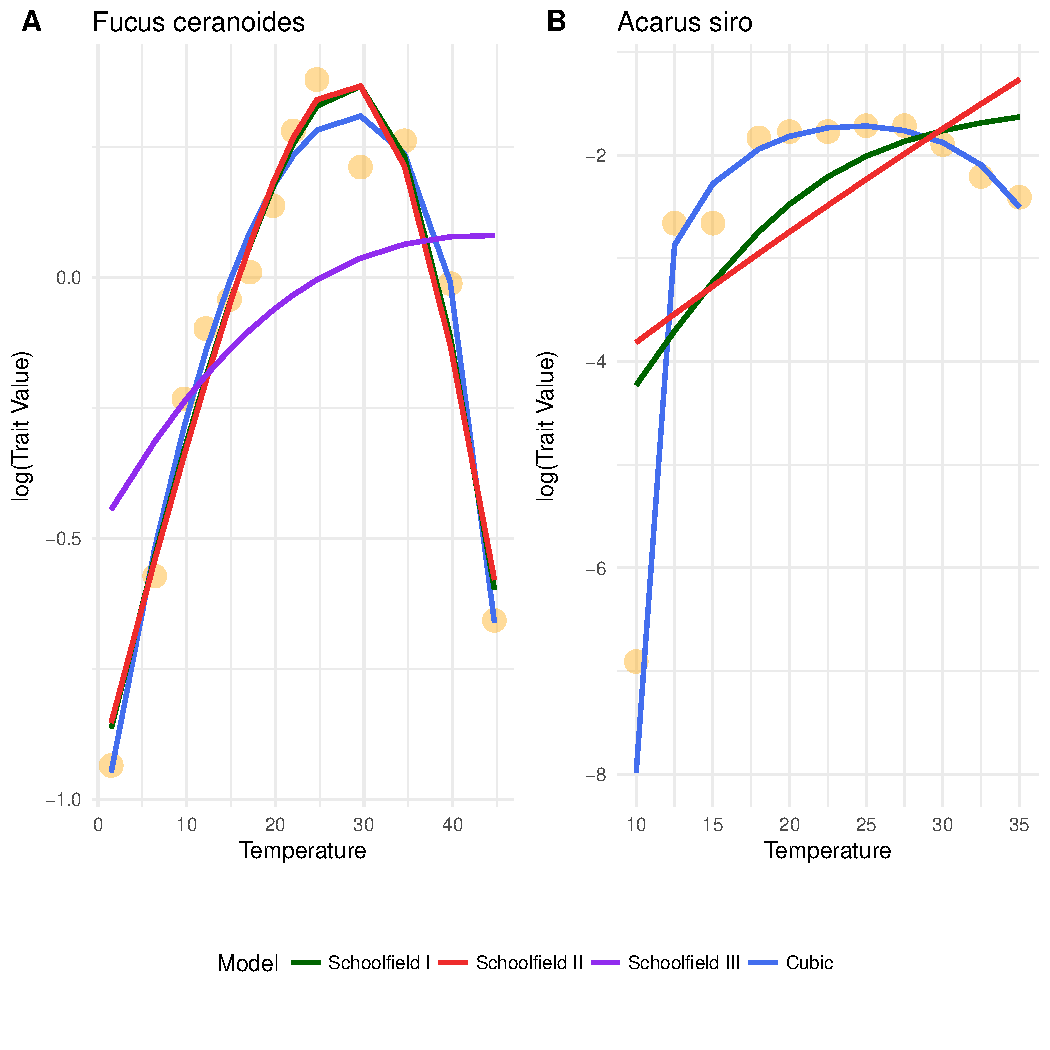
\includegraphics[width=8cm]{Compare_TPC.pdf}
	\captionof{figure}{Two example TPCs. A) A curve where both SI and SII as well as the cubic model capture the general tendency of the data. B) Only the cubic model is able to fit the data adequately.}
\end{center}

In general, the cubic models outperformed the mechanistic ones (Figure 2). When comparing mechanistic models, SII (i.e. the high variation of the Schoolfield model) was the best performing. Surprisingly, the full model fared better than the low-temperature variation  (Figure 2).

\begin{center}
	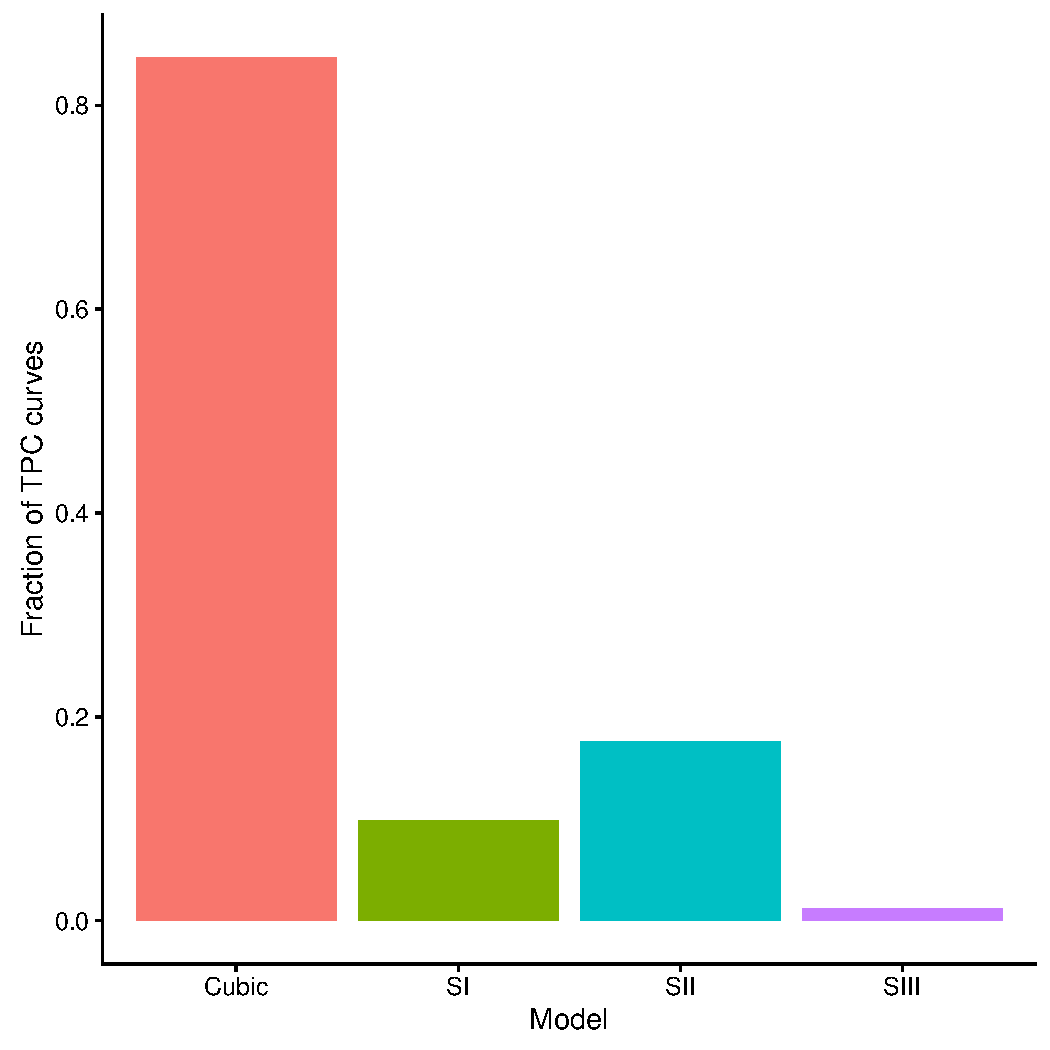
\includegraphics[width=8cm]{compare_models.pdf}
	\captionof{figure}{Overall model performance. The fraction of TPCs for which a model was the best performing is displayed for all fitted models. Models were compared using AICs, significant differences were detected when models had a delta AIC of 2 or more units.}
\end{center}

When comparing how models performed within different consumer habitats, the same general trend is observed (Figure 3). The cubic model consistently outperformed the other mechanistic models. SII consistently performed best for the mechanistic models across habitats.

\begin{center}
	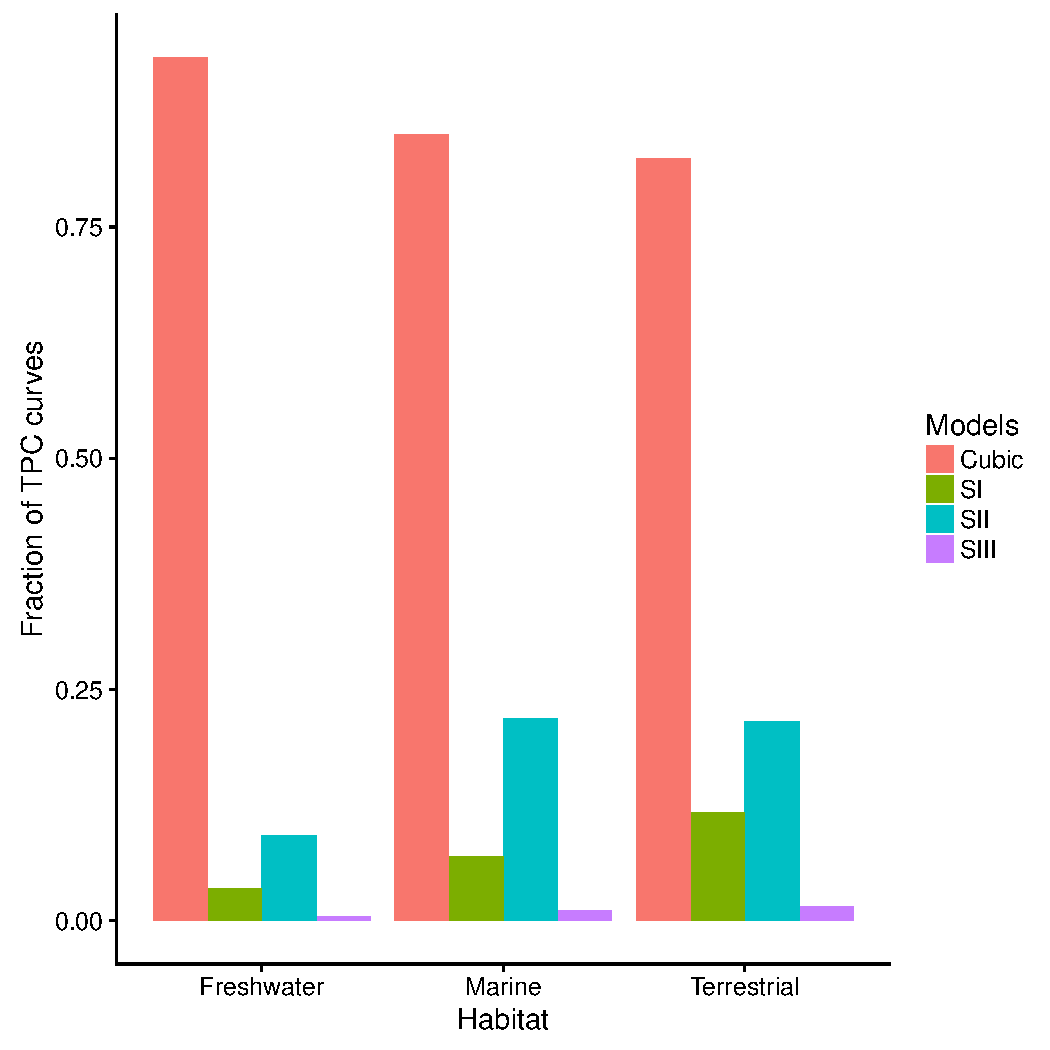
\includegraphics[width=8cm]{Habitat_models.pdf}
	\captionof{figure}{Model performance across habitats. The fraction of TPCs for which a model was the best performing is displayed for freshwater, marine and terrestrial habitats. Models were compared using AICs, significant differences were detected when models had a delta AIC of two or more units. }
\end{center}

Cubic models were found to be the best performing model across all kingdoms (Figure 4). Nevertheless, differences in the performance of the mechanistic models were observed. For the Metazoa kingdom, virtually no mechanistic models outperformed the Cubic ones. Yet, for Monera, Plantae and Protista mechanistic models fared much better. In addition, SI was the best performing mechanistic model for Fungi, reverting previously observed trends  (Figure 4).

\begin{center}
	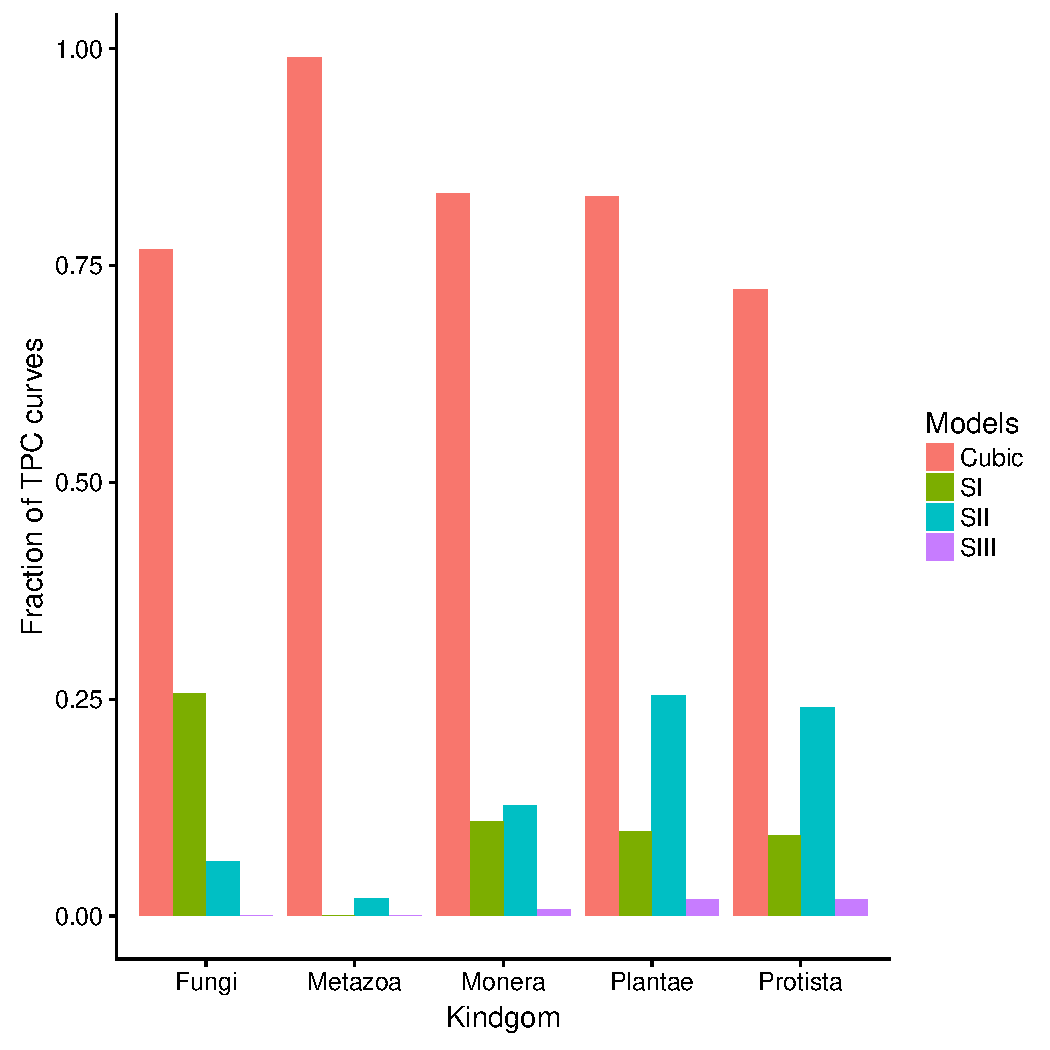
\includegraphics[width=8cm]{Kingdom_models.pdf}
	\captionof{figure}{Model performance across kingdoms. The fraction of TPCs for which a model was the best performing is displayed for the five kingdoms. The Monera kingdom was comprised of both Archea and Bacteria. The Protista kingdom includes Chromista, Protista and Protozoa organisms. Models were compared using AICs, significant differences were detected when models had a delta AIC of two or more units.}
\end{center}

Cubic models yielded the best fits regardless of the type of metabolic trait evaluated (Figure 5). In turn, deterministic models performed best when estimating metabolic trait related to photosynthesis. The lowest performances were recorded for growth related metabolic traits. 

\begin{center}
	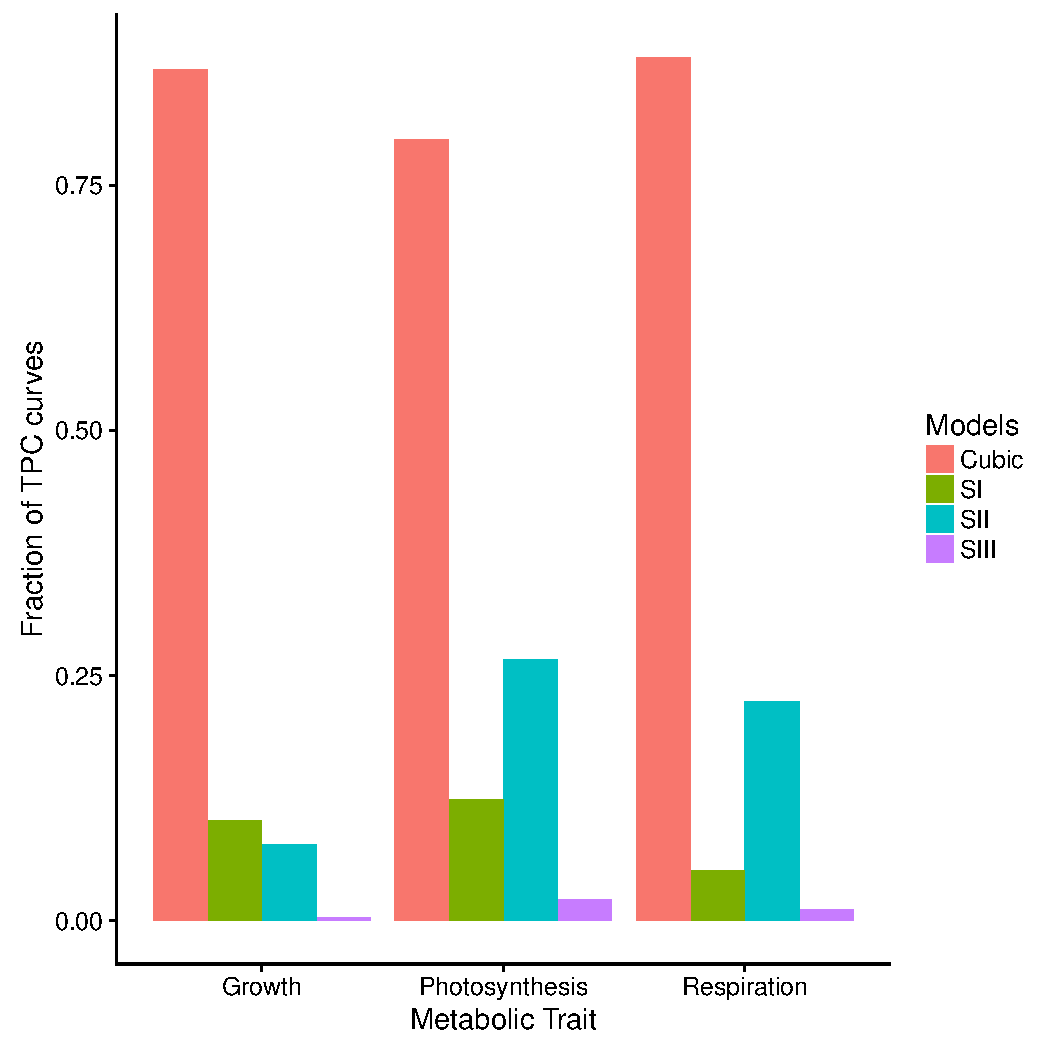
\includegraphics[width=8cm]{Metabolic_models.pdf}
	\captionof{figure}{Model performance across types of metabolic traits. The fraction of TPCs for which a model was the best performing is displayed for growth, photosynthetic and respiration traits. Growth traits include: individual growth rate, individual mass growth rate, population growth rate, radial growth rate and specific growth rate. Photosynthetic traits include: rate of photosynthesis, gross and net photosynthesis. Respiration traits include: mass-specific respiration rate and respiration rate. Models were compared using AICs, significant differences were detected when models had a delta AIC of two or more units.}
\end{center}


%%%%%%%%%% DISCUSSION %%%%%%%%%%%%
%%%%%%%%%%%%%%%%%%%%%%%%%%%%%%

\section*{Discussion}

In general both mechanistic and phenomenological models had a high rate of convergence and seemed to capture the trends  of the TPCs. However, when performing AIC-based model selection cubic models were consistently the best-fitting regardless of the type of metabolic trait measured, the kingdom or habitat of the species to which the TPC corresponded. These results are in sharp contrast to previous findings where Schoolfield models have generated adequate fits. These discrepancies could be due to the sheer diversity of metabolic traits analyzed and the difficulty of estimating adequate initial parameter values, inadequate implementations of fitting algorithms or simply because the mechanistic models failed to adequately explain tendencies. 

\subsection*{Model Performance}

Model convergence was very high in the utilized TPC dataset. Strikingly, nearly all SII and SIII models were able to be fitted to the data. This is indicative that the general structure of the underlying equations do in fact reflect the normal behavior of TPCs. This is why Schoolfield-like models have been widely used to model physiological, ecological and evolutionary traits \cite{Dell,Gillooly,Regniere,Gillooly2,Savage}. As was expected, SI had a lower conversion rate (80\%) possibly due to the difference in the number of estimated parameters when compared to SII, SIII and the cubic models. Thus, for the fitted models it would seem that for each additional estimated parameter we lose 10\% of the convergence rate.

In terms of model performance, cubic models were vastly superior to their mechanistic counterparts. This is possibly due to the fact that phenomenological models do not have a 'constrained' form and thus can more freely adapt to TPC patterns. However, when looking for underlying principles that generate observed patterns, the fact that mechanistic models systematically perform best is discouraging. 

When comparing performance across mechanistic models, SII generally comes on top. This could be indicative of the fact that most TPCs used had high temperature values recorded or because the estimated initial values for \textit{\(E_h\)} and \textit{\(T_h\)} were better than those of \textit{\(E_l\)} and \textit{\(T_l\)}. Moreover, low temperature deactivation of TPCs has been reported to be hard to detect \cite{Pawar}. This could explain the large differences in performance between SII and SIII. SI had a performance which was comparable to SII in some cases (Figure 2 and Figure 4: Monera) and greater than SII in others (Figure 4: Fungi and Figure 5: Growth). Schoolfield models have been previously reported to model growth rates in both fungi and bacteria better than other model types \cite{Gibson,Adair}, which could explain the improvement in performance for both the Fungi kingdom and when modeling growth rates. 

\subsection*{Initial Parameter Estimation and Model Fitting}

Estimation of initial parameters was performed in the same way for all analyzed TPCs. Though this makes approximations a quick process, it could be an inadequate approach for certain datasets. In order to find suitable initial parameter values, a set of assumptions are made about the TPC in question. Namely that the data describe a sigmoid shape with a clearly defined maximum trait value and low trait value at high and low temperatures. However, this was not the case for all TPCs used. In some cases, a maximum trait value was observed at more than one temperature value. When this was occurred, the lowest temperature at which the trait was maximized was defined to be the peak of the curve. However, it could be the case that this was a measuring error and thus the peak trait value was found elsewhere on the curve. Other times, an unrealistic temperature or trait values were found to have been recorded. Evidently this generated over or underestimated initial parameter values. These issues inherently arise when dealing with large and diverse datasets, however in order to maximize the efficiency of mechanistic models to predict TPCs we must be certain that our estimates of initial values are as close to reality as possible. Perhaps comparing the performance of different ways of estimating initial parameter values, like those described by Shi \cite{Shi}, will shed some light on the arduous task that is estimating parameter values from TPCs and make our methods more robust.

Model fitting of mechanistic equations was highly successful (99\% for SII and SIII, 80\% for SI) despite the diversity of measured traits and potentially erroneous estimations of initial parameter values. Nevertheless, for a model to be useful it should also provide meaningful and realistic values of its parameter estimates \cite{Levins}.  The mode of the fitted E values from all three mechanistic models were consistently higher (SI = 1.32, SII = 1.63 and SIII = 5.62) than the reported mean activation of 0.65 across species \cite{Brown}. Moreover, some models estimated activation energy values of up to 900 (kJ/mol). Clearly these estimates are meaningless. These issues could be resolved by setting tougher restrictions on how the model fitting algorithm modifies parameter values. However, if it were the case that biologically meaningless parameter values are systematically produced by a model then the model would have to be reevaluated. A possible solution would be to make the model more parsimonious, as this has been found to be an adequate approach for reducing model over fitting and increasing predictive power \cite{Cox}.

\subsection*{Concluding Remarks}

The reported results are in sharp contrast with previous reports on the accuracy of Schoolfield models to predict TPCs \cite{Padfield,Barneche}. These unexpected findings are likely due to the diversity of trait data used and the one-size-fits-all method of estimating initial parameter values. This in turn likely generated dubious parameter estimates after fitting, which hindered model performance when compared to simple phenomenological models. Though these results may not shed light into the matter of phenomenological vs mechanistic model performance in TPCs, they do highlight the importance of having robust parameter estimation procedures. Schoolfield models are far from perfect \cite{Kontopoulos} and an effort should be made to evaluate how close we are to understanding the mechanistic underpinnings of TPCs.  

\newpage

%%%%%%%%%% REFERENCES %%%%%%%%%%%%
%%%%%%%%%%%%%%%%%%%%%%%%%%%%%%


\bibliography{Mini_project} % reading the Bibtex file 
\bibliographystyle{ieeetr} % sets the referencing by the order in which they were mentioned in the text

\end{document}
